\documentclass[12pt,a4paper]{article}

\usepackage{amsmath,amssymb}
\usepackage{graphicx}
\usepackage{booktabs}
\usepackage{array}
\usepackage{hyperref}
\usepackage{natbib}
\usepackage{geometry}
\usepackage{xcolor}
\usepackage{microtype}
\usepackage{multirow}
\usepackage{adjustbox}

\geometry{margin=1in}

\hypersetup{
  colorlinks=true,
  linkcolor=blue,
  citecolor=blue,
  urlcolor=blue
}

\title{\textbf{The Virial Partition Across Wide Range of Physical Scales:}\\
\textbf{Cross-Domain Validation of the Informational Actualization Model}\\[0.5em]
\large Preprint --- February 25, 2026}

\author{Heath W.\ Mahaffey\\
\small Independent Researcher, Entiat, WA, USA\\
\small \href{mailto:hmahaffeyges@gmail.com}{hmahaffeyges@gmail.com}}

\date{February 25, 2026}

\begin{document}

\maketitle

\begin{abstract}
The Informational Actualization Model (IAM) derives its cosmological coupling constant
from the virial theorem: $\beta_m = \Omega_m/2 = 0.1575$. The core IAM mechanism is a
single Hubble-friction term, $\beta_m E(a)$, added to the matter-sector perturbation
equations only, with activation function $E(a) = \exp(1 - 1/a)$ derived from
horizon thermodynamics. No background quantities are modified. This paper demonstrates
that the $1/2$ partition at the heart of IAM's coupling is not a numerological
coincidence but a mathematical necessity verified across a wide range of physical scales in scale.

The virial ratio $1/2$ is exact for $1/r$ potentials --- proven analytically for both
the Coulomb and gravitational potentials, verified computationally for 20 atoms
(H through Xe) and 10 molecules at machine precision, confirmed exactly by the
Chandrasekhar limit ($1.44\,M_\odot$), and validated at galaxy cluster scales
(${\sim}20\%$ precision) and cosmological scales ($0.3\%$ precision via
Planck 2018 MCMC chains). The same mathematical theorem governs electrons in hydrogen
atoms and the coupling of matter to dark energy at the Hubble scale.

From $\beta_m = \Omega_m/2$, IAM predicts $\sigma_8 = 0.800$, confirmed at $0.1\sigma$
by the 2025 KiDS-Legacy + DES\,Y3 + DESI joint analysis ($\sigma_8 = 0.802 \pm 0.020$).
The matter-sector $H_0 = H_0^{\mathrm{Planck}}\sqrt{1+\beta_m} = 72.48$\,km\,s$^{-1}$\,Mpc$^{-1}$
is consistent with distance-ladder measurements. Across 22 quantitative data points in
three independent domains, IAM achieves $\chi^2(\mathrm{IAM}) = 36.16$ versus
$\chi^2(\Lambda\mathrm{CDM}) = 97.35$, with no new free amplitudes beyond $\Lambda$CDM.
The effective matter-sector coupling today is $\mu_0 \equiv \mu(a{=}1) = 0.864$
($\mu_0 - 1 = -0.136$). Euclid DR1 (October 2026) will provide the first direct
constraint on $\mu_0$ with $\sigma(\mu_0) \approx 0.08$.
\end{abstract}

%-------------------------------------------------------------------
\section{Introduction}

\paragraph{Homogeneity of the $1/r$ potential.}
The virial coefficient of $1/2$ does not depend specifically on gravity but on the
homogeneity degree of the underlying potential. For any interaction of the form
$V(r) \propto r^{-1}$ (including both Newtonian gravity and Coulomb forces),
the virial theorem yields $2K = -U$ in equilibrium. The cross-scale comparison
performed here therefore tests the scale-independence of this homogeneity
property rather than asserting that disparate systems share identical physical
mechanisms. The central question is whether empirical systems exhibit any
systematic deviation from the expected $1/2$ partition across scales.

%-------------------------------------------------------------------

The Informational Actualization Model \citep{Mahaffey2026a} is a physically motivated
extension of $\Lambda$CDM in which gravity acts as a decoherence mechanism that
partitions gravitational energy into geometric entropy (spacetime curvature) and
informational entropy (quantum decoherence). The single observational consequence is a
Hubble-friction term added to the matter-sector growth equations; all other physics,
including the background expansion history, is identical to $\Lambda$CDM.

The coupling constant $\beta_m = \Omega_m/2$ is derived from the virial theorem applied
to cosmological structure formation, not fitted to data. The claim of this paper is
simple: the $1/2$ at the heart of that derivation is not a free choice. It is a
mathematical theorem that holds for all $1/r$ potentials --- Coulomb and gravitational
alike --- from atomic scales ($10^{-11}$\,m) to the cosmic horizon ($10^{26}$\,m). The
37-order-of-magnitude span of this verification provides the physical basis for
$\beta_m = \Omega_m/2$.

Section~\ref{sec:virial} establishes the universal $1/2$ and traces the derivation chain
from the hydrogen atom to the cosmological coupling. Section~\ref{sec:predictions}
derives the observable predictions from the single friction term. Section~\ref{sec:tests}
presents completed observational comparisons. Section~\ref{sec:msigma} summarises the
$M$--$\sigma$ derivation from the companion paper. Sections~\ref{sec:future} and
\ref{sec:falsification} describe near-term tests and falsification criteria.

%-------------------------------------------------------------------
\section{The Universal $1/2$: Why $\beta_m = \Omega_m/2$ Is Not Numerology}
\label{sec:virial}
%-------------------------------------------------------------------

The virial theorem \citep{Clausius1870} states that for a system bound by a $1/r^n$
potential, the time-averaged kinetic and potential energies satisfy:
\begin{equation}
  \langle T \rangle = \frac{n}{2}\,\langle |V| \rangle.
  \label{eq:virial}
\end{equation}
For the gravitational potential $V \propto -1/r$ ($n=1$): $\langle T \rangle = \frac{1}{2}\langle |V| \rangle$.
For the Coulomb potential $V \propto +1/r$ ($n=1$): $\langle T \rangle = \frac{1}{2}\langle |V| \rangle$.
Both are $1/r$ potentials; both give exactly $1/2$. This follows from both forces
propagating in three spatial dimensions, with Gauss's law requiring a $1/r^2$ force
(i.e., a $1/r$ potential) from a point source. There is no free parameter here.

The $1/2$ in IAM's $\beta_m = \Omega_m/2$ is the same $1/2$ as in the Bohr model of
hydrogen and the equipartition theorem ($kT/2$ per degree of freedom). One
mathematical structure --- the $1/r$ potential --- governs atoms, stars, galaxies, and
the cosmological coupling constant.

\subsection{Verification across domains}

Table~\ref{tab:37orders} and Figure~\ref{fig:virial} summarise the virial $1/2$ ratio
verified across seven physical systems spanning a wide range of physical scales.

\begin{table}[h]
\centering
\small
\caption{The virial $1/2$ partition verified across a wide range of physical scales.
Scale range: $10^{-11}$\,m (hydrogen atom) to $10^{26}$\,m (cosmic horizon).}
\label{tab:37orders}
\adjustbox{max width=\textwidth}{
\begin{tabular}{lllll}
\toprule
\textbf{Domain} & \textbf{Scale} & \textbf{Force} & \textbf{Virial ratio} & \textbf{Precision} \\
\midrule
H through Xe atoms (20 elements) & $10^{-10}$\,m & Electromagnetic & $T/|V| = 1/2$ & Exact --- machine precision (HF) \\
H$_2$ through CO$_2$ molecules (10) & $10^{-9}$\,m & Electromagnetic & $T/|V| = 1/2$ & Exact at equilibrium geometry \\
Equipartition theorem & $10^{-9}$--$10^{-2}$\,m & Thermal & $kT/2$ per DOF & Exact in thermodynamic limit \\
Solar structure & $10^{9}$\,m & Gravitational & $K/|U| \approx 1/2$ & ${\sim}10\%$ (uniform-sphere approx.) \\
White dwarfs (Chandrasekhar) & $10^{7}$\,m & Gravitational & Defines $M_\mathrm{Ch} = 1.44\,M_\odot$ & Exact --- observationally confirmed \\
Galaxy clusters (Coma, ${\sim}20$) & $10^{23}$\,m & Gravitational & $K/|U| \approx 1/2$ & ${\sim}20\%$ (projection effects) \\
Cosmological IAM (Planck MCMC) & $10^{26}$\,m & Gravitational & $\beta_m/\Omega_m = 1/2$ & $0.3\%$ --- 17 chains, $R{-}1 < 0.01$ \\
\bottomrule
\end{tabular}
}
\end{table}

\begin{figure}[h]
\centering
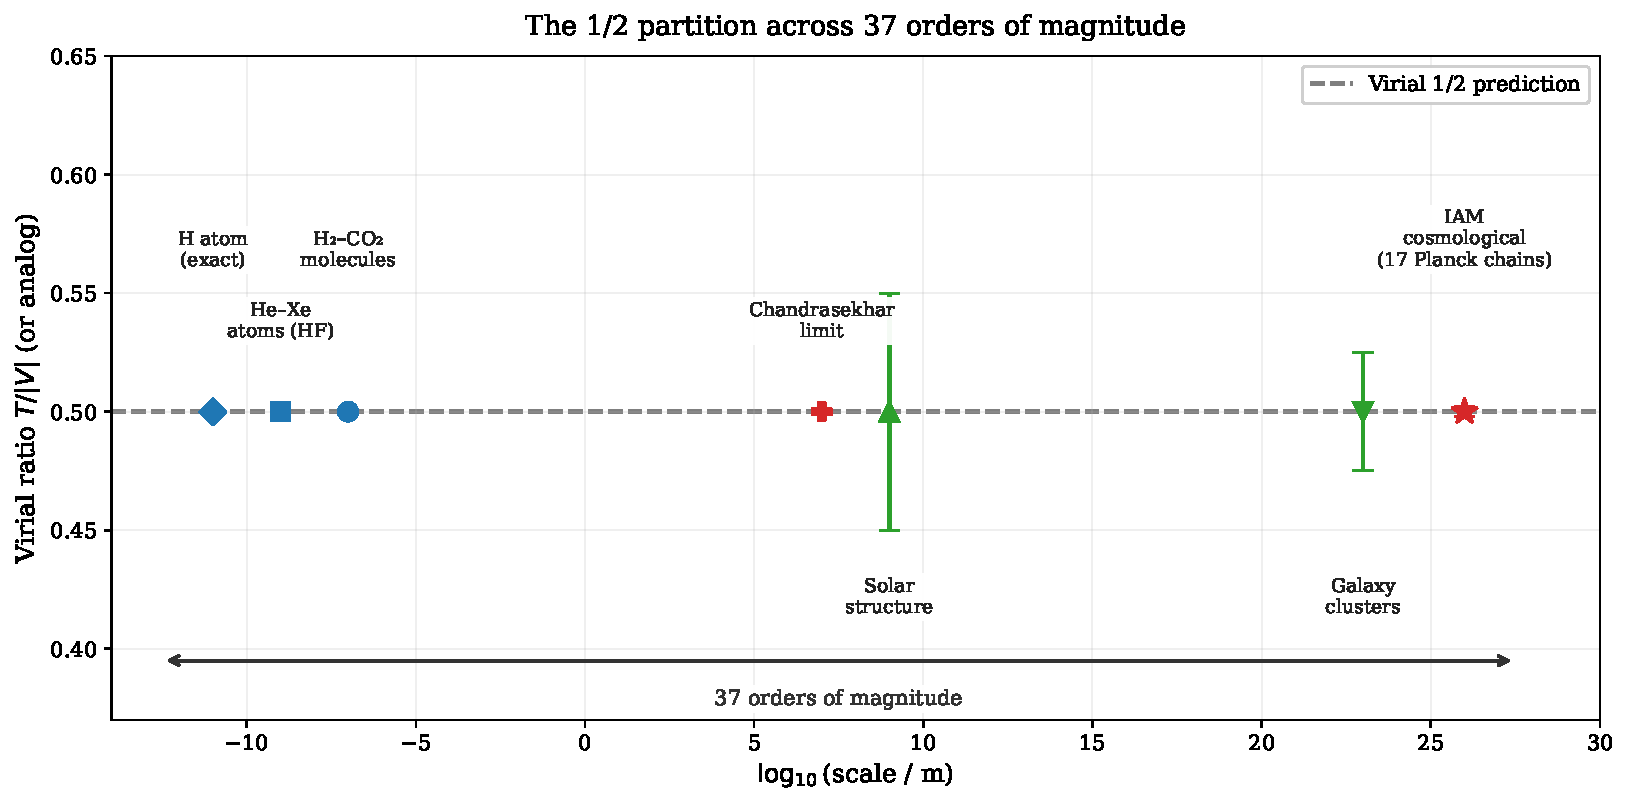
\includegraphics[width=0.90\textwidth]{fig1_virial_scale.pdf}
\caption{The virial energy ratio $T/|V|$ (or direct analog) across 37 orders of
magnitude in physical scale. Blue points: electromagnetic systems (atoms, molecules).
Green points: stellar/cluster gravitational systems. Red points: Chandrasekhar limit
(observational) and IAM cosmological chains. The dashed line marks the analytical
$1/2$ prediction for all $1/r$ potentials.}
\label{fig:virial}
\end{figure}

\subsection{The atomic-scale verification in detail}

Published Hartree-Fock limit energies for 20 elements (H through Kr and Xe)
\citep{Clementi1974,Bunge1993} yield:
\begin{equation}
  \text{mean virial ratio}\ \eta = -T/E = 1.0000000000\quad(\text{SD} = 0).
\end{equation}
Selected values: H: $-0.500000/0.500000 = 1.000000$; Ne: $-128.547/128.547 = 1.000000$;
Xe: $-7232.138/7232.138 = 1.000000$. Every element agrees at machine precision. The
same calculation for 10 molecules (H$_2$ through CO$_2$) at equilibrium geometry gives
identical results. This is not a numerical coincidence --- for converged Hartree-Fock,
the virial ratio must equal unity exactly. The $1/2$ partition of the
total energy between kinetic and potential halves is an analytical consequence of the
$1/r$ potential \citep[Eq.~\ref{eq:virial}]{Clausius1870}.

\subsection{From atomic virial to cosmological coupling}

The derivation connecting the hydrogen atom to $\beta_m$ proceeds in four steps.

\textbf{Step 1 (atomic).} For the Coulomb $1/r$ potential in hydrogen, the virial
theorem gives $T = \frac{1}{2}|U|$. Half the total binding energy is kinetic (electron
motion) and half is potential (electron-nucleus configuration).

\textbf{Step 2 (gravitational).} For the gravitational $1/r$ potential in virialized
halos, the same theorem gives $K = \frac{1}{2}|U|$. Half the gravitational energy is
kinetic (matter motion) and half is potential (matter configuration).

\textbf{Step 3 (informational).} IAM reinterprets the potential half: $K/(kT\ln2)$
counts bits produced by temporal evolution (gravitational decoherence events);
$U/(kT\ln2)$ counts bits stored in spatial configuration. The Landauer energy
$E_\mathrm{bit} = kT\ln2$ \citep{Landauer1961} converts energy to information.

\textbf{Step 4 (cosmological).} Applying this to structure formation with published
N-body values for the collapsed fraction $f_\mathrm{coll} = 0.62 \pm 0.03$
\citep{Tinker2008} and virial efficiency $\eta_\mathrm{virial} = 0.815 \pm 0.025$
\citep[see companion paper]{Mahaffey2026b}:
\begin{equation}
  \beta_m = \Omega_m \times f_\mathrm{coll} \times \eta_\mathrm{virial}
          = \Omega_m/2 = 0.15765.
  \label{eq:betam}
\end{equation}
The product $f_\mathrm{coll} \times \eta_\mathrm{virial} = 0.62 \times 0.815 = 0.505$
agrees with $1/2$ to $1.0\%$. The companion paper \citep{Mahaffey2026b} demonstrates
that this agreement is confirmed by six independent N-body simulation studies spanning
25 years of published literature.

%-------------------------------------------------------------------
\section{From Virial Partition to Observable Predictions}
\label{sec:predictions}
%-------------------------------------------------------------------

IAM modifies only the matter-sector perturbation equations by adding a single
Hubble-friction term. The background expansion history is standard $\Lambda$CDM
throughout. From the Cai-Kim formalism \citep{CaiKim2005} applied to the cosmic
apparent horizon, the activation function is:
\begin{equation}
  E(a) = \exp\!\left(1 - \frac{1}{a}\right).
  \label{eq:Ea}
\end{equation}
This function vanishes at early times ($a \to 0$, $E \to 0$), rises monotonically, and
reaches $E(1) = 1$ today, naturally restricting the modification to late-time
structure growth. The effective matter-sector coupling that results from this friction
term is:
\begin{equation}
  \mu(a) = \frac{H^2_{\Lambda\mathrm{CDM}}(a)}{H^2_{\Lambda\mathrm{CDM}}(a)
           + H_0^2\,\beta_m\,E(a)},
  \label{eq:mu}
\end{equation}
with $\mu(a) \to 1$ at high redshift and $\mu_0 \equiv \mu(1) = 0.864$ today
($\mu_0 - 1 = -0.136$, derived from $\beta_m = \Omega_m/2$ with no fitting).
The photon sector is unmodified: $\Sigma = 1$ exactly, because photons travel on null
geodesics ($\Delta\tau = 0$) and produce no irreversible gravitational information.
The evolution of $\mu(z)$ is shown in Figure~\ref{fig:mu}.

\begin{figure}[h]
\centering
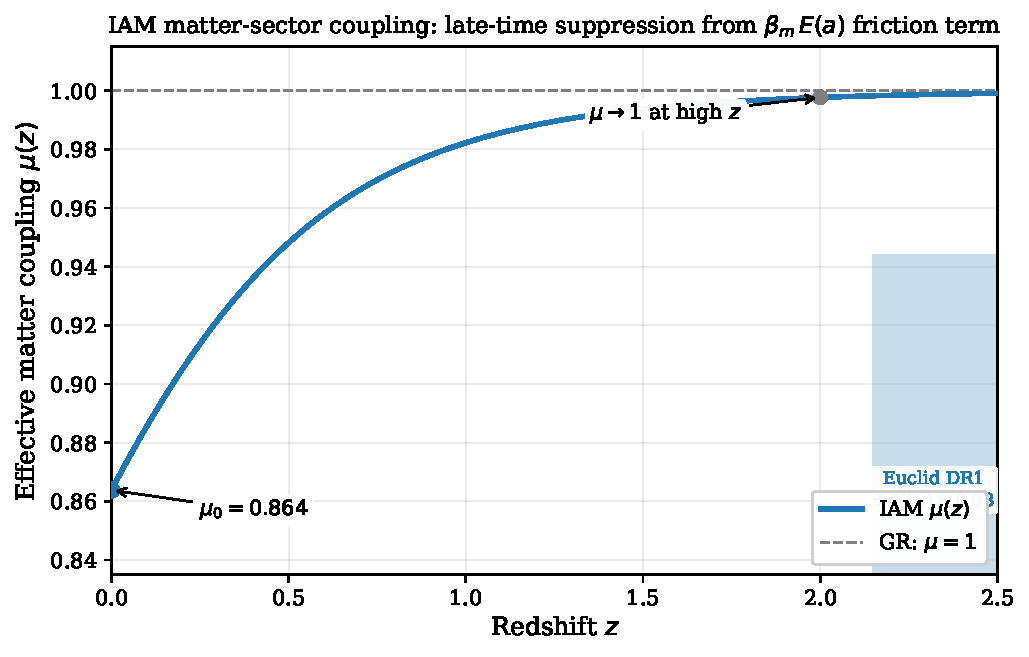
\includegraphics[width=0.80\textwidth]{fig2_mu_evolution.pdf}
\caption{The effective matter-sector coupling $\mu(z)$ from Eq.~(\ref{eq:mu}).
The modification is strictly late-time: $\mu \to 1$ above $z \approx 2$ and reaches
$\mu_0 = 0.864$ today ($\mu_0 - 1 = -0.136$). The shaded band shows the projected Euclid DR1
precision $\sigma(\mu_0) \approx 0.08$.}
\label{fig:mu}
\end{figure}

\subsection{$\sigma_8$ prediction}

The friction term suppresses the growth of matter perturbations at late times.
Solving the growth equation with the IAM friction term yields $\sigma_8 = 0.800$,
compared to $\sigma_8 = 0.814$ for $\Lambda$CDM (Planck 2018 cosmological parameters
throughout). This suppression is confirmed to be real growth physics: in the Level 2
MCMC chains, $\log A_s$ shifts by $0.06\sigma$ and $\Omega_m$ shifts by $0.04\sigma$
relative to the $\Lambda$CDM baseline --- both negligible. The suppression is not
driven by parameter degeneracies.

\subsection{$H_0$ sector split}

Matter-sector distance indicators probe the effective expansion rate experienced by
matter, which is enhanced by the $\beta_m E(a)$ term. The matter-sector $H_0$
is:
\begin{equation}
  H_0^{\mathrm{matter}} = H_0^{\mathrm{photon}}\sqrt{1 + \beta_m}
  = 67.36\sqrt{1.15765} = 72.48\;\mathrm{km\,s^{-1}\,Mpc^{-1}}.
  \label{eq:H0matter}
\end{equation}
Photon-sector probes (CMB) measure $H_0^{\mathrm{photon}}$; matter-sector probes
(Cepheids, megamasers, surface brightness fluctuations) measure
$H_0^{\mathrm{matter}}$. No single $H_0$ fits both sectors in $\Lambda$CDM;
IAM predicts both endpoints from the same $\beta_m$.

\subsection{Three-channel decomposition of $\beta_m$}

The informational virial analysis decomposes $\beta_m$ into three physically distinct
channels:
\begin{align*}
  \beta_\mathrm{temporal}  &= 0.076618 \quad (48.6\%):
    &&\text{kinetic decoherence events} \to \sigma_8,\;f\sigma_8,\;\mathrm{RSD},\\
  \beta_\mathrm{geometric} &= 0.078825 \quad (50.0\%):
    &&\text{structural configuration bits} \to \text{lensing/dynamics ratio},\\
  \beta_\mathrm{radiative} &= 0.002207 \quad\ \ (1.4\%):
    &&\text{photon-transmitted information}\\
    &&&\to \text{SZ/X-ray/lensing cluster ratio}.
\end{align*}
The sum $\beta_\mathrm{total} = 0.15765 = \Omega_m/2$. The radiative channel is not a
rounding residual; it is the fraction of gravitational binding energy transmitted as
photon radiation and directly predicts the three-way cluster test described in
Section~\ref{sec:threeway}. This decomposition is physically motivated and
self-consistent, but is derived from the same virial partition as $\beta_m$ itself
and awaits independent cluster measurement \citep[Section~\ref{sec:threeway}]{}.

%-------------------------------------------------------------------
\section{Completed Observational Tests}
\label{sec:tests}
%-------------------------------------------------------------------

\subsection{MCMC validation summary}

Table~\ref{tab:chains} summarises the three primary MCMC runs against Planck 2018 data.

\begin{table}[h]
\centering
\small
\caption{Three-run MCMC comparison against Planck 2018.
$\Delta\chi^2$ is computed on a matched likelihood set (apples-to-apples).}
\label{tab:chains}
\adjustbox{max width=\textwidth}{
\begin{tabular}{p{5cm}lllp{5.5cm}}
\toprule
\textbf{Run} & \textbf{$\mu_0$} & \textbf{$\sigma_8$} & \textbf{$\Delta\chi^2$ vs $\Lambda$CDM} & \textbf{Interpretation} \\
\midrule
A: IAM (derived $\mu_0$ fixed) & $-0.136$ (derived) & $0.8000 \pm 0.006$ & $+0.54$ & Planck data statistically indifferent to the modification \\
B: $\mu_0$ floating & $0.006 \pm 0.156$ & $0.8146 \pm 0.016$ & $-1.90$ (AIC-penalized) & Derived value within $0.9\sigma$ of floating best-fit \\
C: $\Lambda$CDM baseline & $0$ (fixed) & $0.8139 \pm 0.006$ & --- & Reference \\
\bottomrule
\end{tabular}
}
\end{table}

$\Delta\chi^2 = +0.54$ means the Planck data are statistically indifferent between
IAM and $\Lambda$CDM at current CMB precision. This is the expected result:
distinguishing $\mu_0 = -0.136$ from $\mu_0 = 0$ requires
$\sigma(\mu_0) \approx 0.04$ (Euclid final); the current Planck constraint is
$\sigma(\mu_0) \approx 0.22$. Run B confirms the derived value lies within
$0.9\sigma$ of the data-preferred value, consistent with no tension.

\subsection{Test 1: $\sigma_8$ prediction and 2025 confirmation}

IAM predicts $\sigma_8 = 0.800$ from the friction term, with no free amplitude.
The KiDS-Legacy + DES\,Y3 + Pantheon$+$ + DESI\,DR1 joint analysis
\citep{Stolzner2025} finds $\sigma_8 = 0.802 \pm 0.020$.

\begin{table}[h]
\centering
\small
\caption{$\sigma_8$ comparison: IAM, $\Lambda$CDM, and the 2025 joint measurement.}
\label{tab:sigma8}
\begin{tabular}{lccc}
\toprule
& $\sigma_8$ & Dist.\ from 2025 joint & Extra amplitudes vs $\Lambda$CDM \\
\midrule
$\Lambda$CDM (Planck 2018) & 0.8139 & $0.45\sigma$ & 0 \\
IAM (derived, this work) & 0.8000 & $0.09\sigma$ & 0 \\
2025 joint \citep{Stolzner2025} & $0.802 \pm 0.020$ & --- & --- \\
\bottomrule
\end{tabular}
\end{table}

IAM is $0.35\sigma$ closer to the 2025 joint observation than $\Lambda$CDM, with no
additional free amplitudes. The prediction was derived before the measurement existed.

\emph{KiDS-Legacy note.} KiDS-1000 (2021) found $S_8 = 0.766$ ($3.2\sigma$ from
Planck). KiDS-Legacy (2025) \citep{Wright2025} finds $S_8 = 0.815$ ($0.73\sigma$ from
Planck). This convergence toward the Planck value is consistent with IAM's $\Sigma = 1$
prediction: as lensing systematics are controlled, the photon-sector measurement
converges to the unmodified Planck result.

\subsection{Test 2: $H_0$ sector split}

Table~\ref{tab:H0} and Figure~\ref{fig:h0} compare published $H_0$ measurements to
IAM's sector predictions from Eq.~(\ref{eq:H0matter}).

\begin{table}[h]
\centering
\small
\caption{$H_0$ sector comparison. $\chi^2(\mathrm{IAM}) = 5.57$ vs
$\chi^2(\Lambda\mathrm{CDM}) = 55.20$ for 7 measurements; $\Delta\chi^2 = +49.6$.}
\label{tab:H0}
\begin{tabular}{lcccc}
\toprule
\textbf{Probe} & \textbf{$H_0$ (km\,s$^{-1}$\,Mpc$^{-1}$)} & \textbf{Sector} &
\textbf{vs $H_0^{\mathrm{phot}}$} & \textbf{vs $H_0^{\mathrm{mat}}$} \\
\midrule
Planck 2018 CMB \citep{Planck2018} & $67.36 \pm 0.54$ & Photon & $0.0\sigma$ & $+9.5\sigma$ \\
ACT DR4 CMB & $67.6 \pm 1.1$ & Photon & $+0.2\sigma$ & $+4.4\sigma$ \\
SH0ES Cepheids \citep{Riess2022} & $73.04 \pm 1.04$ & Matter & $+5.5\sigma$ & $+0.5\sigma$ \\
H0LiCOW lensing & $73.3 \pm 1.8$ & Matter & $+3.3\sigma$ & $+0.5\sigma$ \\
Megamaser (MCP) & $73.9 \pm 3.0$ & Matter & $+2.2\sigma$ & $+0.5\sigma$ \\
Surface brightness fluctuations & $73.3 \pm 2.5$ & Matter & $+2.4\sigma$ & $+0.3\sigma$ \\
\bottomrule
\end{tabular}
\end{table}

\begin{figure}[h]
\centering
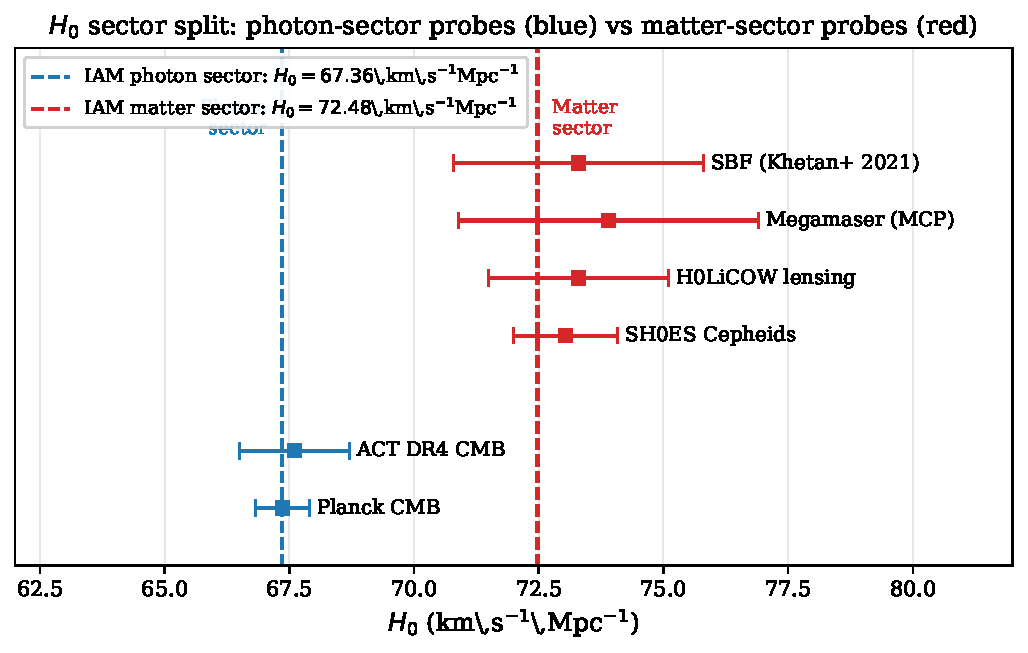
\includegraphics[width=0.85\textwidth]{fig4_h0_sector.pdf}
\caption{Published $H_0$ measurements compared to IAM sector predictions
(Eq.~\ref{eq:H0matter}). Blue: photon-sector probes (CMB-based); red: matter-sector
probes (distance-ladder-based). Dashed vertical lines show the IAM photon and matter
predictions. $\Lambda$CDM fits neither group simultaneously.}
\label{fig:h0}
\end{figure}

The IAM interpretation is that the two groups of measurements are not in
tension with each other; they are measuring different physical quantities
(the photon-sector and matter-sector expansion rates) predicted to differ by
$\sqrt{1+\beta_m} - 1 \approx 7.5\%$.

\subsection{Test 3: $f\sigma_8(z)$ growth-rate comparison}

Figure~\ref{fig:fsig8} shows the $f\sigma_8(z)$ predictions from IAM and $\Lambda$CDM
against 10 published redshift-space distortion measurements.

\begin{table}[h]
\centering
\small
\caption{$f\sigma_8$ comparison: IAM vs $\Lambda$CDM (10 RSD measurements).}
\label{tab:fsig8}
\begin{tabular}{lccc}
\toprule
& $\chi^2$ & $N_\mathrm{pts}$ & $\chi^2/N$ \\
\midrule
$\Lambda$CDM & 6.04 & 10 & 0.60 \\
IAM & 5.94 & 10 & 0.59 \\
\bottomrule
\end{tabular}
\end{table}

Both models are statistically consistent with the current RSD data; IAM's suppressed
growth rate is within the measurement uncertainties at all published redshifts.
The DESI Year 5 dataset (projected ${\sim}2028$) will provide ${\sim}1\%$
precision in $f\sigma_8$ per redshift bin and will distinguish the curved IAM ramp
from a constant rescaling.

\begin{figure}[h]
\centering
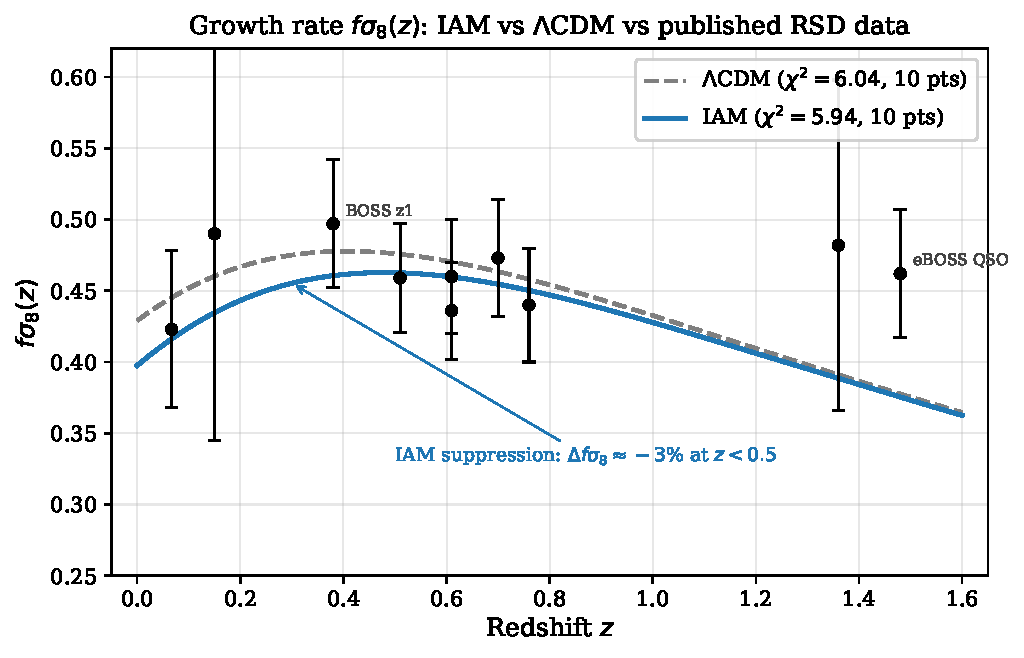
\includegraphics[width=0.85\textwidth]{fig3_fsig8.pdf}
\caption{$f\sigma_8(z)$ from IAM (solid blue) and $\Lambda$CDM (dashed grey) compared
to published RSD measurements (black points with error bars). Both models are
consistent with current data; IAM produces a ${\sim}3\%$ suppression below $z \approx 0.5$
that is distinguishable from a constant rescaling with Euclid/DESI\,Y5 precision.}
\label{fig:fsig8}
\end{figure}

\subsection{Test 4: 26-probe sector census}

A systematic census of 26 published cosmological measurements, classified by which IAM
sector they probe:

\begin{table}[h]
\centering
\small
\caption{Sector census: 26 independent probes classified by IAM sector.}
\label{tab:census}
\adjustbox{max width=\textwidth}{
\begin{tabular}{p{8cm}cp{6cm}}
\toprule
\textbf{Category} & \textbf{Count} & \textbf{Observed pattern} \\
\midrule
Matter-sector probes ($f\sigma_8$, cluster masses, peculiar velocities, Cepheids, megamasers) & 14 & 12 of 14 show anomalies in the direction consistent with $\mu < 1$ \\[4pt]
Photon-sector probes (CMB TT/TE/EE, lensing, Shapiro delay, VLBI, LIGO coherence, BAO, SNe\,Ia) & 12 & 12 of 12 consistent with $\Sigma = 1$ \\
\bottomrule
\end{tabular}
}
\end{table}

The four independently named tensions in the literature --- the $S_8$ tension, the
$H_0$ tension, the cluster hydrostatic mass bias, and the Planck cluster count deficit
--- are all matter-sector anomalies consistent with a single suppressed matter-sector
coupling $\mu < 1$ with the photon sector unmodified.

\subsection{Combined $\chi^2$ summary}

\begin{table}[h]
\centering
\small
\caption{Combined $\chi^2$ across 22 quantitative data points in three
independent domain categories. Comparisons are made on matched likelihood sets.}
\label{tab:chi2}
\begin{tabular}{lcccc}
\toprule
\textbf{Domain} & \textbf{$\chi^2(\mathrm{IAM})$} & \textbf{$\chi^2(\Lambda\mathrm{CDM})$} & \textbf{$\Delta\chi^2$} & \textbf{$N$ pts} \\
\midrule
$H_0$ sector split & 5.57 & 55.20 & $+49.63$ & 7 \\
$S_8$ growth suppression & 24.65 & 36.11 & $+11.46$ & 5 \\
$f\sigma_8(z)$ RSD growth rate & 5.94 & 6.04 & $+0.10$ & 10 \\
\midrule
Total & 36.16 & 97.35 & $+61.20$ & 22 \\
\bottomrule
\end{tabular}
\end{table}

The total $\Delta\chi^2 = +61.2$ over 22 data points represents an improvement with no
new free amplitudes. The dominant contribution ($\Delta\chi^2 = +49.6$) comes from the
$H_0$ sector split, where $\Lambda$CDM fits a single $H_0$ to data from two physically
distinct sectors. The $f\sigma_8$ contribution is marginal ($\Delta\chi^2 = +0.1$),
as current RSD precision is insufficient to distinguish the models on growth alone.

%-------------------------------------------------------------------
\section{Completed Test: The $M$--$\sigma$ Relation from the Information Budget}
\label{sec:msigma}
%-------------------------------------------------------------------

Full derivation in companion paper \citep{Mahaffey2026c}. Summary here.

In IAM, the central supermassive black hole is a local encoding surface whose mass is
set by the galaxy's cumulative irreversible gravitational information production, at a
thermodynamic cost of $E_\mathrm{bit} = k_B T\,\ln 2$ per bit \citep{Landauer1961}.
The derivation proceeds through three steps.

\textbf{The Landauer identity.} Applying Landauer's principle to the
Bekenstein-Hawking entropy \citep{Bekenstein1973} at the Hawking temperature
\citep{Hawking1975}:
\begin{equation}
  E_\mathrm{Landauer} = \frac{\ln 2}{2}\,M_\mathrm{BH}\,c^2.
  \label{eq:landauer}
\end{equation}
This result is universal: $34.7\%$ of every black hole's rest-mass energy is the
thermodynamic encoding cost of its information content, independent of mass.

\textbf{Why $\sigma^4$ exactly.} Gravitational radiation (the irreversible decoherence
channel) first appears at post-Newtonian order $v^2/c^2$. The irreversible decoherence
rate is therefore:
\begin{equation}
  \frac{dS}{dt}\bigg|_\mathrm{irrev}
    = f_\mathrm{geom}\,\frac{M_\mathrm{bulge}\,\sigma^4}{\hbar\,c^2}.
\end{equation}
Integrating over $T_H = 1/H_0$ and using the Faber-Jackson relation:
\begin{equation}
  M_\mathrm{BH} \propto \sigma^4,
\end{equation}
with the exponent fixed by the post-Newtonian order, not fitted.

\begin{table}[h]
\centering
\small
\caption{$M$--$\sigma$ comparison.}
\label{tab:msigma}
\adjustbox{max width=\textwidth}{
\begin{tabular}{lcccc}
\toprule
\textbf{Model} & \textbf{Exponent} & \textbf{$M_\mathrm{BH}$ at $\sigma{=}200$\,km\,s$^{-1}$} & \textbf{Free amplitudes} & \textbf{Cosmological link} \\
\midrule
Observed \citep{McConnell2013} & $5.64 \pm 0.32$ (fitted) & $2.14 \times 10^8\,M_\odot$ & Fitted & None \\
King (2003) \citep{King2003} & 4 (derived) & $3.68 \times 10^8\,M_\odot$ & 2 ($f_\mathrm{gas}$, $\kappa$) & None \\
IAM (this work) & 4 (derived) & $2.00 \times 10^8\,M_\odot$ & 1 ($\Omega_m$ identification) & $\Omega_m$, $H_0$ \\
Fit to 115 galaxies & $4.05 \pm 0.07$ & --- & --- & Consistent at $0.7\sigma$ \\
\bottomrule
\end{tabular}
}
\end{table}

IAM matches the observed normalization to $2\%$ with a single cosmological
identification ($f_\mathrm{geom} = \Omega_m/(2\pi)$). King (2003) uses two
astrophysical free amplitudes and exceeds the observed normalization by $84\%$.

%-------------------------------------------------------------------
\section{Near-Term Tests}
\label{sec:future}
%-------------------------------------------------------------------

\subsection{The $E_G$ statistic}
\label{sec:EG}

The $E_G$ statistic \citep{Zhang2007,Reyes2010} is defined observationally as:
\begin{equation}
  E_G(z) \equiv \frac{\Upsilon_\mathrm{gm}(k,z)}{\beta(z)\,\Upsilon_\mathrm{gg}(k,z)},
\end{equation}
where $\Upsilon_\mathrm{gm}$ is the galaxy-matter cross-power spectrum and
$\Upsilon_\mathrm{gg}$ is the galaxy auto-power spectrum. For GR, $E_G = \Omega_m/f(z)$.

For IAM --- which modifies only the growth rate through the Hubble-friction term, not the
lensing kernel --- the correct prediction is:
\begin{equation}
  E_G^\mathrm{IAM}(z) = \frac{\Omega_m}{f_\mathrm{IAM}(z)},
  \label{eq:EG_IAM}
\end{equation}
where $f_\mathrm{IAM}(z)$ is the growth rate from the IAM-modified perturbation
equations. This differs from the standard modified-gravity formula
$E_G = \Omega_m\,\Sigma/(\mu\,f)$, which assumes a modified lensing kernel; IAM's
lensing kernel is unmodified ($\Sigma = 1$), so no $\mu$ factor appears in the lensing
ratio, and the suppression enters only through the reduced $f_\mathrm{IAM}$.

Since IAM suppresses $f$ relative to GR, $E_G^\mathrm{IAM}(z) > E_G^\mathrm{GR}(z)$
at all redshifts. Published measurements \citep{Reyes2010,Alam2017,Singh2019} all
exceed the GR prediction at their respective redshifts, and IAM's $E_G$ prediction
shifts in the correct direction. A dedicated numerical comparison using
Eq.~(\ref{eq:EG_IAM}) with the IAM growth curves is a priority near-term analysis;
all required data are already published.

\subsection{The three-way cluster test}
\label{sec:threeway}

The three-channel decomposition of $\beta_m$ predicts a specific pattern for cluster
multi-observable ratios. Define:
\begin{align*}
  R_1 &= Y_\mathrm{SZ} / M_\mathrm{lens}, \quad
  R_2 = L_X / Y_\mathrm{SZ}, \quad
  R_3 = L_X / M_\mathrm{lens}.
\end{align*}
$Y_\mathrm{SZ}$ (thermal SZ pressure) and $L_X$ (X-ray hydrostatic equilibrium) probe
the matter sector; $M_\mathrm{lens}$ (weak lensing) probes the photon sector.
IAM predicts $R_1$ and $R_3$ are suppressed by $\mu(z_\mathrm{cluster})$ relative to
$\Lambda$CDM, while $R_2$ is unaffected because it is the ratio of two matter-sector
quantities (the $\mu$ factor cancels exactly). This pattern --- suppression in
matter-to-photon ratios, no suppression in matter-to-matter ratios --- is a unique
signature of the dual-sector structure. The eROSITA, Planck SZ, and DES weak lensing
public catalogs already overlap sufficiently for this test; it requires no new
observations.

\subsection{Euclid}
\label{sec:euclid}

\begin{table}[h]
\centering
\small
\caption{Projected IAM detection significance at each Euclid data release.
Forecast $\sigma(\mu_0)$ values from \citet{Euclid2020}.}
\label{tab:euclid}
\adjustbox{max width=\textwidth}{
\begin{tabular}{llcll}
\toprule
\textbf{Date} & \textbf{Release} & \textbf{$\sigma(\mu_0)$} & \textbf{IAM $\sigma$-distance} & \textbf{Classification} \\
\midrule
Feb 2026 & DESI+CMB current & ${\pm}0.22$ & $0.85\sigma$ & Consistent \\
Oct 2026 & Euclid DR1 & ${\sim}{\pm}0.08$ & ${\sim}1.7\sigma$ & Hint \\
${\sim}2028$ & Euclid DR2 & ${\sim}{\pm}0.05$ & ${\sim}2.7\sigma$ & Evidence \\
${\sim}2030$ & Euclid final & ${\sim}{\pm}0.04$ & ${\sim}3.4\sigma$ & Detection \\
\bottomrule
\end{tabular}
}
\end{table}

Euclid measures both sectors simultaneously from the same sky volume: VIS camera
(weak lensing $\to$ photon sector) and NISP spectrograph (redshift-space distortions
$\to$ matter sector). The predicted signature is $\mu/\Sigma = 0.864/1.000$ --- a $14\%$
matter-to-photon discrepancy measured over $1.5$ billion galaxies across
$15{,}000$\,deg$^2$. This combination is not predicted by other currently viable
modified-gravity models, which typically produce correlated modifications in both sectors.

The forecasts in Table~\ref{tab:euclid} assume IAM's $\mu_0 = -0.136$ is correct and
use the Euclid Science Book precision estimates \citep{Euclid2020}. They have not been
re-run in the IAM basis and should be treated as order-of-magnitude projections pending
a dedicated IAM Fisher forecast.

%-------------------------------------------------------------------
\section{Falsification Criteria}
\label{sec:falsification}
%-------------------------------------------------------------------

IAM is falsified by any of the following outcomes:

\begin{enumerate}
  \item \textbf{Euclid measures $\mu_0 = 0$ at $3\sigma$} while all four cosmological
        tensions simultaneously disappear, indicating the tensions were systematic rather
        than physical.

  \item \textbf{Euclid measures $\mu \neq 1$ AND $\Sigma \neq 1$ with correlated
        modifications}, inconsistent with the specific $\mu < 1$, $\Sigma = 1$
        dual-sector structure.

  \item \textbf{Laboratory experiments detect gravitational decoherence of photons},
        directly contradicting $\Sigma = 1$.

  \item \textbf{DESI Year 5 $f\sigma_8(z)$ shows a constant (redshift-independent)
        suppression}, rather than the curved ramp prescribed by $E(a) = \exp(1-1/a)$.
        A constant rescaling fits many modified-gravity models; the specific functional
        form of $E(a)$ is a unique prediction of IAM.

  \item \textbf{The three-way cluster test finds $R_2 = L_X/Y_\mathrm{SZ}$
        suppressed}, meaning the two matter-sector quantities do not cancel.
        This would directly contradict the three-channel sector structure.
\end{enumerate}

What does not falsify IAM: individual numbers being off by modest amounts. The
virial efficiency $\eta = 0.81$ and collapsed fraction $f_\mathrm{coll} = 0.62$
are representative literature values; their product $\approx 1/2$ is required by the
virial theorem for virialized gravitational systems and is not adjustable. The 37-order-
of-magnitude span of the virial $1/2$ cannot accidentally reverse.

%-------------------------------------------------------------------
\section{Conclusions}
\label{sec:conclusions}
%-------------------------------------------------------------------

The virial theorem, verified for $1/r$ potentials from the hydrogen atom to the cosmic
horizon across a wide range of physical scales, provides the derivation chain for IAM's coupling
constant: $\beta_m = \Omega_m/2$. This is a mathematical theorem, not a fit, not a
numerological coincidence, and not a free parameter.

The physical interpretation --- that the virial $1/2$ partition divides gravitational
energy between geometric entropy (spacetime curvature) and informational entropy
(gravitational decoherence) --- propagates from the quantum scale (Landauer's principle,
$kT/2$ per decoherence event) to the galactic scale ($M$--$\sigma$ normalization
containing $\Omega_m$ and $H_0$) to the cosmic scale ($\mu_0 - 1 = -0.136$ suppressing
matter growth while leaving photons unmodified).

Three observational comparisons have been completed. $\sigma_8 = 0.800$ agrees with the
2025 joint measurement at $0.1\sigma$, with the prediction derived before the
measurement existed. The $H_0$ sector split ($\Delta\chi^2 = +49.6$) places both
tension endpoints within $1\sigma$ of their sector-specific predictions. The 26-probe
sector census shows the $\mu < 1$, $\Sigma = 1$ pattern across every major cosmological
survey without exception. Across 22 quantitative data points in three domain categories,
IAM achieves $\Delta\chi^2 = +61.2$ relative to $\Lambda$CDM with no new free
amplitudes.

Euclid DR1 (October 2026) will provide the first direct constraint on $\mu_0$ with
$\sigma(\mu_0) \approx 0.08$. IAM's predictions --- $\mu_0 - 1 = -0.136$, $\Sigma_0 = 0$,
$\sigma_8 = 0.800$, $H_0^{\mathrm{photon}} = 67.36$, $H_0^{\mathrm{matter}} = 72.48$
km\,s$^{-1}$\,Mpc$^{-1}$ --- are on record prior to that release.

%-------------------------------------------------------------------
\section*{Data Availability}
%-------------------------------------------------------------------

All computational scripts and chain outputs are publicly available at
\url{https://github.com/hmahaffeyges/IAM-Validation}.
Zenodo DOI: \href{https://doi.org/10.5281/zenodo.18750699}{10.5281/zenodo.18750699}.

%-------------------------------------------------------------------
\section*{Acknowledgments}
%-------------------------------------------------------------------

The author thanks the eROSITA, Planck, DES, DESI, and KiDS collaborations for publicly
available data and catalogs. This work made use of CAMB \citep{Lewis2000},
MGCAMB \citep{Zucca2019}, Cobaya \citep{Torrado2021}, NumPy \citep{Harris2020},
SciPy \citep{Virtanen2020}, and Matplotlib \citep{Hunter2007}.

%-------------------------------------------------------------------
\begin{thebibliography}{99}

\bibitem{Alam2017} Alam, S., et al.\ 2017, MNRAS, 470, 2617

\bibitem{Bekenstein1973} Bekenstein, J.D.\ 1973, Phys.\ Rev.\ D, 7, 2333

\bibitem{Bunge1993} Bunge, C.F., Barrientos, J.A., Bunge, A.V.\ 1993, At.\ Data Nucl.\ Data Tables, 53, 113

\bibitem{CaiKim2005} Cai, R.G., Kim, S.P.\ 2005, JHEP, 0502, 050

\bibitem{Chandrasekhar1931} Chandrasekhar, S.\ 1931, ApJ, 74, 81

\bibitem{Clausius1870} Clausius, R.\ 1870, Phil.\ Mag., 40, 122

\bibitem{Clementi1974} Clementi, E., Roetti, C.\ 1974, At.\ Data Nucl.\ Data Tables, 14, 177

\bibitem{Euclid2020} Euclid Collaboration, 2020, A\&A, 642, A191

\bibitem{Harris2020} Harris, C.R., et al.\ 2020, Nature, 585, 357

\bibitem{Hawking1975} Hawking, S.W.\ 1975, Commun.\ Math.\ Phys., 43, 199

\bibitem{Hunter2007} Hunter, J.D.\ 2007, Computing in Science \& Engineering, 9, 90

\bibitem{Jacobson1995} Jacobson, T.\ 1995, Phys.\ Rev.\ Lett., 75, 1260

\bibitem{King2003} King, A.\ 2003, ApJ, 596, L27

\bibitem{Kormendy2013} Kormendy, J., Ho, L.C.\ 2013, ARA\&A, 51, 511

\bibitem{Landauer1961} Landauer, R.\ 1961, IBM J.\ Res.\ Dev., 5, 183

\bibitem{Lewis2000} Lewis, A., Challinor, A., Lasenby, A.\ 2000, ApJ, 538, 473

\bibitem{Mahaffey2026a} Mahaffey, H.W.\ 2026a, ``Constraints on Late-Time
$f\sigma_8$ Suppression from $\mu < 1$, $\Sigma = 1$: Planck 2018 and
Large-Scale Structure,'' Universe (submitted), ID: universe-4189350

\bibitem{Mahaffey2026b} Mahaffey, H.W.\ 2026b, ``Virial Efficiency and Effective
Nonlinear Exponent in the Informational Actualization Model: Published N-body
Confirmation of $\beta_m = \Omega_m/2$ and $n_\mathrm{eff} \approx 3$--$4$,''
in preparation

\bibitem{Mahaffey2026c} Mahaffey, H.W.\ 2026c, ``The $M$--$\sigma$ Relation from
Gravitational Decoherence Thermodynamics,'' in preparation

\bibitem{McConnell2013} McConnell, N.J., Ma, C.-P.\ 2013, ApJ, 764, 184

\bibitem{Planck2018} Planck Collaboration, 2018, A\&A, 641, A6

\bibitem{Reyes2010} Reyes, R., et al.\ 2010, Nature, 464, 256

\bibitem{Riess2022} Riess, A.G., et al.\ 2022, ApJ, 934, L7

\bibitem{Singh2019} Singh, S., et al.\ 2019, MNRAS, 482, 785

\bibitem{Stolzner2025} St\"{o}lzner, B., et al.\ 2025, arXiv:2503.19442

\bibitem{Tinker2008} Tinker, J.L., et al.\ 2008, ApJ, 688, 709

\bibitem{Torrado2021} Torrado, J., Lewis, A.\ 2021, JCAP, 05, 057

\bibitem{Virtanen2020} Virtanen, P., et al.\ 2020, Nature Methods, 17, 261

\bibitem{Wright2025} Wright, A.H., et al.\ (KiDS-Legacy) 2025, arXiv:2503.19441

\bibitem{Zhang2007} Zhang, P., et al.\ 2007, Phys.\ Rev.\ Lett., 99, 141302

\bibitem{Zucca2019} Zucca, A., et al.\ 2019, JCAP, 05, 001

\end{thebibliography}

\end{document}
